\documentclass[../main.tex]{subfiles}
\graphicspath{{\subfix{../Images/}}}

\begin{document}

\chapter{Transformations}

When you write vertex or fragment programs, it is important to understand the coordinate systems that you are working with. This chapter explains the transformations that take place in the graphics pipeline, without going into detail about the underlying mathematics. The chapter has the following two sections:

\begin{itemize}
\item \textbf{"Coordinate Systems"} explains the various coordinate systems used to represent vertex positions as they are transformed prior to rasterization.
\item \textbf{"Applying the Theory"} describes how to apply the theory of coordinate systems and matrices in Cg.
\end{itemize}

\section{4.1 Coordinate Systems}

The purpose of the graphics pipeline is to create images and display them on your screen. The graphics pipeline takes geometric data representing an object or scene (typically in three dimensions) and creates a two-dimensional image from it. Your application supplies the geometric data as a collection of vertices that form polygons, lines, and points. The resulting image typically represents what an observer or camera would see from a particular vantage point.

As the geometric data flows through the pipeline, the GPU's vertex processor transforms the constituent vertices into one or more different coordinate systems, each of which serves a particular purpose. Cg vertex programs provide a way for you to program these transformations yourself.

Vertex programs may perform other tasks, such as lighting (discussed in Chapter 5) and animation (discussed in Chapter 6), but transforming vertex positions is a task \textit{required} by all vertex programs. You cannot write a vertex program that does not output a transformed position, because the rasterizer needs transformed positions in order to assemble primitives and generate fragments.

So far, the vertex program examples you've encountered limited their position processing to simple 2D transformations. This chapter explains how to implement conventional 3D transformations to render 3D objects.

Figure \ref{fig:4-1} illustrates the conventional arrangement of transforms used to process vertex positions. The diagram annotates the transitions between each transform with the coordinate space used for vertex positions as the positions pass from one transform to the next.

The following sections describe each coordinate system and transform in this sequence. We assume that you have some basic knowledge of matrices and transformations, and so we explain each stage of the pipeline with a high-level overview.

\begin{figure}
    \centering
    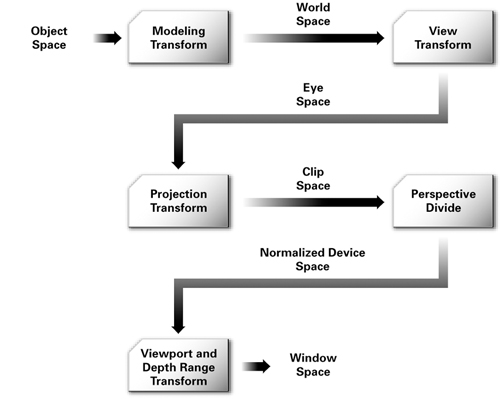
\includegraphics[width=1\linewidth]{fig4_1.jpg}
    \caption{Figure 4-1 Coordinate Systems and Transforms for Vertex Processing}
    \label{fig:4-1}
\end{figure}

\subsection{4.1.1 Object Space}

Applications specify vertex positions in a coordinate system known as \textit{object space} (also called \textit{model space}). When an artist creates a 3D model of an object, the artist selects a convenient orientation, scale, and position with which to place the model's constituent vertices. The object space for one object may have no relationship to the object space of another object. For example, a cylinder may have an object-space coordinate system in which the origin lies at the center of the base and the z direction points along the axis of symmetry.

You represent each vertex position, whether in object space or in one of the subsequent spaces, as a vector. Typically, your application maintains each object-space 3D vertex position as an $<x, y, z>$ vector. Each vertex may also have an accompanying object-space surface normal, also stored as an $<x, y, z>$ vector.

\subsection{4.1.2 Homogeneous Coordinates}

More generally, we consider the $<x, y, z>$ position vector to be merely a special case of the four-component $<x, y, z, w>$ form. This type of four-component position vector is called a \textit{homogeneous position}. When we express a vector position as an $<x, y, z>$ quantity, we assume that there is an implicit 1 for its \textit{w} component.

Mathematically, the \textit{w} value is the value by which you would divide the \textit{x}, \textit{y}, and \textit{z} components to obtain the conventional 3D (nonhomogeneous) position, as shown in Equation 4-1.

\FloatBarrier
\begin{equationcaption}
$
\langle \frac{x}{w},\frac{y}{w},\frac{z}{w},1 \rangle = \langle x,y,z,w \rangle
$
\caption{Equation 4-1 Converting Between Nonhomogeneous and Homogeneous Positions}
\end{equationcaption}
\FloatBarrier

Expressing positions in this homogeneous form has many advantages. For one, multiple transformations, including projective transformations required for perspective 3D views, can be combined efficiently into a single 4x4 matrix. This technique is explained in Section 4.2. Also, using homogeneous positions makes it unnecessary to perform expensive intermediate divisions and to create special cases involving perspective views. Homogeneous positions are also handy for representing directions and curved surfaces described by rational polynomials.

We will return to the \textit{w} component when discussing the projection transform.

\subsection{4.1.3 World Space}

Object space for a particular object gives it no spatial relationship with respect to other objects. The purpose of \textit{world space} is to provide some absolute reference for all the objects in your scene. How a world-space coordinate system is established is arbitrary. For example, you may decide that the origin of world space is the center of your room. Objects in the room are then positioned relative to the center of the room and some notion of scale (Is a unit of distance a foot or a meter?) and some notion of orientation (Does the positive y-axis point "up"? Is north in the direction of the positive x-axis?).

\subsection{4.1.4 The Modeling Transform}

The way an object, specified in object space, is positioned within world space is by means of a modeling transform. For example, you may need to rotate, translate, and scale the 3D model of a chair so that the chair is placed properly within your room's world-space coordinate system. Two chairs in the same room may use the same 3D chair model but have different modeling transforms, so that each chair exists at a distinct location in the room.

You can mathematically represent all the transforms in this chapter as a 4x4 matrix. Using the properties of matrices, you can combine several translations, rotations, scales, and projections into a single 4x4 matrix by multiplying them together. When you concatenate matrices in this way, the combined matrix also represents the combination of the respective transforms. This turns out to be very powerful, as you will see.

If you multiply the 4x4 matrix representing the modeling transform by the object-space position in homogeneous form (assuming a 1 for the \textit{w} component if there is no explicit \textit{w} component), the result is the same position transformed into world space. This same matrix math principle applies to all subsequent transforms discussed in this chapter.

Figure \ref{fig:4-2} illustrates the effect of several different modeling transformations. The left side of the figure shows a robot modeled in a basic pose with no modeling transformations applied. The right side shows what happens to the robot after you apply a series of modeling transformations to its various body parts. For example, you must rotate and translate the right arm to position it as shown. Further transformations may be required to translate and rotate the newly posed robot into the proper position and orientation in world space.
\begin{figure}
    \centering
    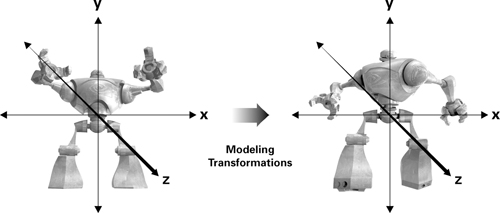
\includegraphics[width=1\linewidth]{fig4_2.jpg}
    \caption{Figure 4-2 The Effect of Modeling Transformations}
    \label{fig:4-2}
\end{figure}

\subsection{4.1.5 Eye Space}

Ultimately, you want to look at your scene from a particular viewpoint (the "eye"). In the coordinate system known as \textit{eye space} (or \textit{view space}), the eye is located at the origin of the coordinate system. Following the standard convention, you orient the scene so the eye is looking down one direction of the \textit{z}-axis. The "up" direction is typically the positive \textit{y} direction.

Eye space, which is particularly useful for lighting, will be discussed in Chapter 5.

\subsection{4.1.6 The View Transform}

The transform that converts world-space positions to eye-space positions is the \textit{view transform}. Once again, you express the view transform with a 4x4 matrix.

The typical view transform combines a translation that moves the eye position in world space to the origin of eye space and then rotates the eye appropriately. By doing this, the view transform defines the position and orientation of the viewpoint.

\begin{figure}
    \centering
    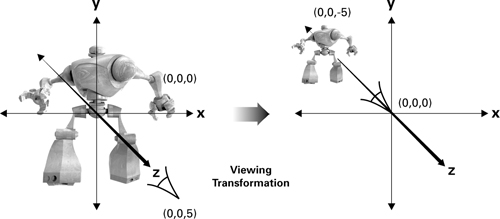
\includegraphics[width=1\linewidth]{fig4_3.jpg}
    \caption{Figure 4-3 The Effect of the Viewing Transformation}
    \label{fig:4-3}
\end{figure}

Figure \ref{fig:4-3} illustrates the view transform. The left side of the figure shows the robot from Figure 4-2 along with the eye, which is positioned at $<0, 0, 5>$ in the world-space coordinate system. The right side shows them in eye space. Observe that eye space positions the origin at the eye. In this example, the view transform translates the robot in order to move it to the correct position in eye space. After the translation, the robot ends up at $<0, 0, -5>$ in eye space, while the eye is at the origin. In this example, eye space and world space share the positive \textit{y}-axis as their "up" direction and the translation is purely in the \textit{z} direction. Otherwise, a rotation might be required as well as a translation.

\subsection*{The Modelview Matrix}

Most lighting and other shading computations involve quantities such as positions and surface normals. In general, these computations tend to be more efficient when performed in either eye space or object space. World space is useful in your application for establishing the overall spatial relationships between objects in a scene, but it is not particularly efficient for lighting and other shading computations.

For this reason, we typically combine the two matrices that represent the modeling and view transforms into a single matrix known as the \textit{modelview matrix}. You can combine the two matrices by simply multiplying the view matrix by the modeling matrix.

\subsection{4.1.7 Clip Space}

Once positions are in eye space, the next step is to determine what positions are actually viewable in the image you eventually intend to render. The coordinate system subsequent to eye space is known as \textit{clip space}, and coordinates in this space are called \textit{clip coordinates}.

The vertex position that a Cg vertex program outputs is in clip space. Every vertex program optionally outputs parameters such as texture coordinates and colors, but a vertex program \textit{always} outputs a clip-space position. As you have seen in earlier examples, the \textbf{POSITION} semantic is used to indicate that a particular vertex program output is the clip-space position.

\subsection{4.1.8 The Projection Transform}

The transform that converts eye-space coordinates into clip-space coordinates is known as the \textit{projection transform}.

The projection transform defines a \textit{view frustum} that represents the region of eye space where objects are viewable. Only polygons, lines, and points that are within the view frustum are potentially viewable when rasterized into an image. OpenGL and Direct3D have slightly different rules for clip space. In OpenGL, everything that is viewable must be within an axis-aligned cube such that the \textit{x}, \textit{y}, and \textit{z} components of its clip-space position are less than or equal to its corresponding \textit{w} component. This implies that $-w \leq x \leq w$, $-w \leq y \leq w$, and $-w \leq z \leq w$. Direct3D has the same clipping requirement for \textit{x} and \textit{y}, but the \textit{z} requirement is $0 \leq z \leq w$. These clipping rules assume that the clip-space position is in homogeneous form, because they rely on \textit{w}.

The projection transform provides the mapping to this clip-space axis-aligned cube containing the viewable region of clip space from the viewable region of eye space—otherwise known as the view frustum. You can express this mapping as a 4x4 matrix.

\subsection*{The Projection Matrix}

The 4x4 matrix that corresponds to the projection transform is known as the \textit{projection matrix}.

Figure \ref{fig:4-4} illustrates how the projection matrix transforms the robot in eye space from Figure \ref{fig:4-3} into clip space. The entire robot fits into clip space, so the resulting image should picture the robot without any portion of the robot being clipped.

\begin{figure}
    \centering
    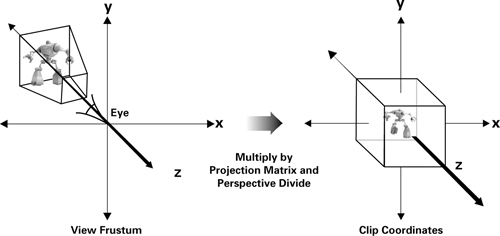
\includegraphics[width=1\linewidth]{fig4_4.jpg}
    \caption{Figure 4-4 The Effect of the Projection Matrix}
    \label{fig:4-4}
\end{figure}

The clip-space rules are different for OpenGL and Direct3D and are built into the projection matrix for each respective API. As a result, if Cg programmers rely on the appropriate projection matrix for their choice of 3D programming interface, the distinction between the two clip-space definitions is not apparent. Typically, the application is responsible for providing the appropriate projection matrix to Cg programs.

\subsection{4.1.9 Normalized Device Coordinates}

Clip coordinates are in the homogenous form of $<x, y, z, w>$, but we need to compute a 2D position (an \textit{x} and \textit{y} pair) along with a depth value. (The depth value is for \textit{depth buffering}, a hardware-accelerated way to render visible surfaces.)

\subsection*{Perspective Division}

Dividing \textit{x}, \textit{y}, and \textit{z} by \textit{w} accomplishes this. The resulting coordinates are called \textit{normalized device coordinates}. Now all the visible geometric data lies in a cube with positions between $<-1, -1, -1>$ and $<1, 1, 1>$ in OpenGL, and between $<-1, -1, 0>$ and $<1, 1, 1>$ in Direct3D.

The 2D vertex programs in Chapters 2 and 3 output what you now know as normalized device coordinates. The 2D output position in these examples assumed an implicit \textit{z} value of 0 and a \textit{w} value of 1.

4.1.10 Window Coordinates
The final step is to take each vertex's normalized device coordinates and convert them into a final coordinate system that is measured in pixels for \textit{x} and \textit{y}. This step, called the \textit{viewport transform}, feeds the GPU's rasterizer. The rasterizer then forms points, lines, or polygons from the vertices, and generates fragments that determine the final image. Another transform, called the \textit{depth range transform}, scales the \textit{z} value of the vertices into the range of the depth buffer for use in depth buffering.

\section{4.2 Applying the Theory}

Despite all the discussion about coordinate spaces, the Cg code you need for transforming vertices correctly is quite trivial. Normally, the vertex program receives vertex positions in object space. The program then multiplies each vertex by the modelview and projection matrices to get that vertex into clip space. In practice, you would concatenate these two matrices so that just one multiplication is needed instead of two. Figure \ref{fig:4-5} illustrates this principle by showing two ways to get from object coordinates to clip coordinates.

\begin{figure}
    \centering
    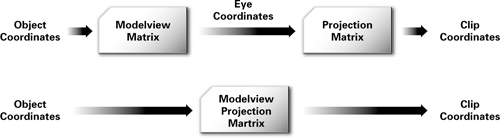
\includegraphics[width=1\linewidth]{fig4_5.jpg}
    \caption{Figure 4-5 Optimizations for Transforming to Clip Space}
    \label{fig:4-5}
\end{figure}

Example 4-1 shows how a typical Cg program would efficiently handle 3D vertex transformations from object space directly to clip space.

\FloatBarrier
\begin{lstlisting}[caption=Example 4-1. The \textbf{C4E1v_transform} Vertex Program]
void C4E1v_transform(float4 position  : POSITION,
                 out float4 oPosition : POSITION,
             uniform float4x4 modelViewProj)
{
  // Transform position from object space to clip space
  oPosition = mul(modelViewProj, position);
}
\end{lstlisting}
\FloatBarrier

The program takes the object-space position (\textbf{position}) and concatenated modelview and projection matrices (\textbf{modelViewProj}) as input parameters. Your OpenGL or Direct3D application would be responsible for providing this data. There are Cg runtime routines that help you load the appropriate matrix based on the current OpenGL or Direct3D transformation state. The \textbf{position} parameter is then transformed with a matrix multiplication, and the result is written out to \textbf{oPosition}:

\FloatBarrier
\begin{lstlisting}
   // Transform position from object space to clip space
   oPosition = mul(modelViewProj, position);
\end{lstlisting}
\FloatBarrier

In this book, we explicitly assign all output parameters, even if they are simply being passed through. We use the "\textbf{o}" prefix to differentiate input and output parameters that have the same names.

\section{4.3 Exercises}

\begin{enumerate}
\item \textbf{Answer this:} List the various coordinate spaces and the sequence of transformations used to move from one to the next.
\item \textbf{Answer this:} If you are interested in the theory of transformations, list some situations where you can use just a 3x3 matrix for the modelview and projection matrices instead of a complete 4x4 matrix.
\item \textbf{Try this yourself:} Use \textbf{cgc} to output the vertex program assembly for the \textbf{C4E1v_transform} example. The \textbf{DP4} instruction computes a four-component dot product. How many such instructions are generated by the program's \textbf{mul} routine?
\end{enumerate}

\section{4.4 Further Reading}

Computer graphics textbooks explain vertex transformation and develop more of the matrix math underlying the topic than presented here. We recommend Edward Angel's \textit{Interactive Computer Graphics: A Top-Down Approach with OpenGL, Third Edition} (Addison-Wesley, 2002).

If you want to develop your intuition for the projective transformations that underlie vertex transformation and be entertained at the same time, read \textit{Jim Blinn's Corner: A Trip Down the Graphics Pipeline} (Morgan Kaufmann, 1996).

\textit{Graphics Gems} (Academic Press, 1994), edited by Andrew Glassner, has many useful short articles about modeling, transformation, and matrix techniques.

\end{document}